\section{Introdução}

\subsection{Motivação}

Quando há transferência de calor através da fronteira comum entre dois corpos materiais em contato físico, observa-se experimentalmente que nessa interface há
uma descontinuidade no perfil de temperatura, ou seja, o contato térmico nessa região não é perfeito \citep{livro_ozisik}. 
Esse fenômeno ocorre devido à combinação dos efeitos de três componentes \citep{livro_madhusudana}:
\begin{itemize}
  \item Condução de calor através dos pontos em que há contato efetivo sólido-sólido, devido à presença de irregularidades microscópicas e macroscópicas;
  \item Condução de calor através do meio intersticial, preenchido por algum fluido (por exemplo, ar) ou vácuo;
  \item Radiação de calor, que é desprezada na maioria das aplicações. 
\end{itemize} 


% 
% Na maioria das aplicações, os efeitos de radiação são desprezados, bem como  Mesmo a altas pressões, o fenômeno da descontinuidade de temperatura permanece relevante, pois a
% superfície efetiva de contato não coincide com a superfície total de contato.

A figura \ref{fig1} ilustra o processo de transferência de calor através da interface de contato entre dois sólidos. As linhas de fluxo de calor
sofrem uma \textit{constrição} nos pontos de contato; nos espaços entre os pontos, devido às dimensões das lacunas da ordem de micrômetros, a convecção
de calor é desconsiderada em detrimento da condução.

\begin{figure}[h!b]
\begin{center}
\begin{tikzpicture}
\node at (0, 0)
	{
		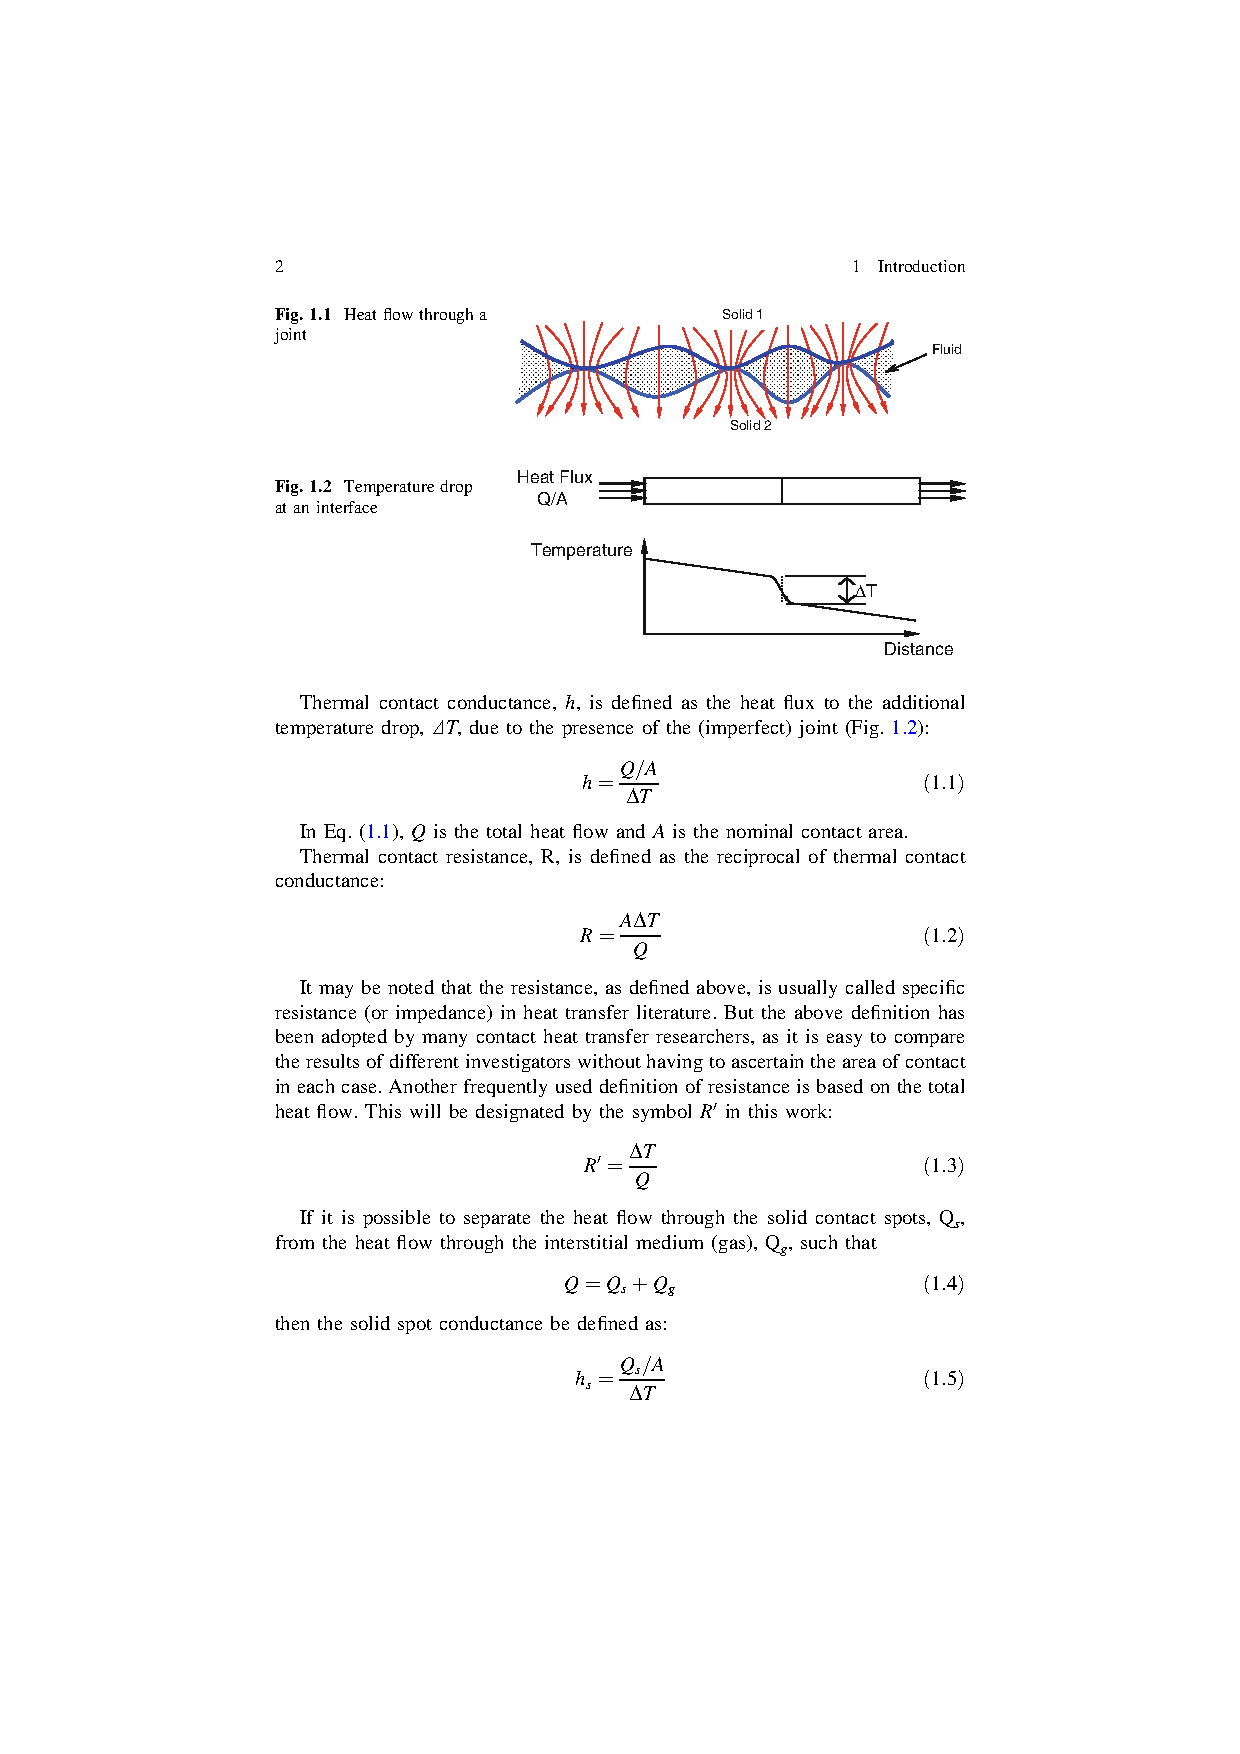
\includegraphics[trim=250 642 150 154, clip=true]{img/img1.pdf}
	};
	
\node[scale=0.8] at (0, 0.9) {Sólido 1};
\node[scale=0.8] at (0, -1.1) {Sólido 2};
\node[scale=0.8] at (4, 0.3) {Fluido};
\end{tikzpicture}
\caption{Transferência de calor através da interface entre dois corpos (adaptado de \citeauthor{livro_ozisik}, \citeyear{livro_ozisik})}
\label{fig1}
\end{center}
\end{figure}

A \textit{condutância térmica de contato} -- abreviada como CTC -- é definida como sendo a razão entre o fluxo de calor e o salto de temperatura
devido à presença do contato imperfeito \citep{livro_madhusudana}:
\begin{equation}
	h_c = \frac{Q_c/A}{\Delta T_c} = \frac{q_c}{\Delta T_c} \label{eq:definicao_1}
\end{equation}
onde $Q_C$ é o fluxo total de calor através da interface, $A$ é a área de contato nominal ou aparente, $q_c$ é o fluxo de calor por unidade de área e e $\Delta T_c$ é o salto de temperatura na interface. As unidades
da CTC são as mesmas do coeficiente de transferência de calor por convecção ($W/m^2 K$ no SI).

A inversa da CTC é denominada \textit{resistência térmica de contato} (RTC):
\begin{equation}
	R_c = \frac{1}{h_c} = \frac{A\Delta T_c}{Q_c} = \frac{\Delta T_c}{q_c}
\end{equation}

Uma definição equivalente da CTC pode ser formulada a partir da análise do problema de condução de calor no domínio constituído pelos
corpos em contato, através das condições de contorno avaliadas na interface de contato \citep{livro_ozisik}. Nessa região, pode-se afirmar que o fluxo
de calor saindo ou entrando em cada um dos sólidos deve se igualar ao fluxo de calor através da interface.

Sejam, portanto, $T_1$ e $T_2$ os campos de temperatura em cada um dos sólidos cuja interface é representada na figura \ref{fig1}. Sejam $k_1$ e $k_2$
as respectivas condutividades térmicas dos sólidos, e seja $q_c$ o fluxo de calor por unidade de área através da interface de contato. Assim, o balanço de energia permite escrever:
\begin{equation}
	q_c = -k_1\frac{\partial T_1}{\partial \mathbf{n}_1}\bigg|_i
	=
	h_c(T_1 - T_2)_i
	=
	k_2\frac{\partial T_2}{\partial \mathbf{n}_2}\bigg|_i \label{eq:definicao_2}
\end{equation}
De onde se obtém:
\begin{equation}
	h_c = \frac{-k_1\displaystyle\frac{\partial T_1}{\partial \mathbf{n}_1}\bigg|_i}{(T_1 - T_2)_i} = \frac{k_2\displaystyle\frac{\partial T_2}{\partial \mathbf{n}_2}\bigg|_i}{(T_1 - T_2)_i} \label{eq:definicao_3}
\end{equation}
Os gradientes de temperatura são calculados sobre as direções dos vetores normais
$\mathbf{n}_1$ e $\mathbf{n}_2$, que apontam para fora das fronteiras que delimitam os corpos materiais correspondentes; em particular,
na interface de contato teremos $\mathbf{n}_2 = -\mathbf{n}_1$. O subscrito $i$ indica que todas as avaliações são feitas sobre a superfície de contato.

Nota-se facilmente a partir da equação \eqref{eq:definicao_3} que a CTC é uma propriedade não necessariamente constante ao longo da interface de contato,
uma vez que tanto o fluxo de calor como o salto entre as temperaturas podem variar em cada ponto sobre a interface. De fato, nos locais onde a diferença é nula (ou seja, o contato
é perfeito), a CTC assumiria valor infinito, ou alternativamente, a RTC seria nula. No outro extremo, havendo uma região micrométrica perfeitamente
isolante entre os corpos materiais, o fluxo de calor seria nulo para uma diferença de temperatura finita; ali a CTC seria nula, equivalente a um valor
infinito de RTC. Assim, a CTC também pode ser entendida como um parâmetro de avaliação da qualidade do contato entre dois corpos materiais.

O levantamento da CTC também permite avaliar qualitativamente a presença de descontinuidades ou falhas
em materiais homogêneos, uma vez que, devido aos saltos de temperatura provocados pela interface de contato no local da falha,
o campo de temperatura medido na superfície externa fornece resultados diferentes do esperado se tais falhas não ocorressem.

A necessidade de cálculo ou estimativa da CTC se faz presente em diversas aplicações, como por exemplo, na área aeroespacial \citep{artigo_aerospacial}, microeletrônica
\citep{artigo_snaith}, ou no projeto de trocadores de calor \citep{artigo_huang}. Para tanto, podem ser aplicados métodos de medição que normalmente exigem
algum conhecimento de detalhes das superfícies de contato, tais como rugosidade ou aspereza, e necessitam de tomadas de temperatura no interior dos corpos em contato, levando a arranjos
experimentais complexos ou intrusivos. Conhecidas (ou estimadas por regressão) as temperaturas na interface e o fluxo de calor por unidade de área, a aplicação
direta da definição permite levantar a CTC, normalmente como um valor médio sobre a interface. Essa foi a abordagem adotada na maioria dos problemas de estimativa
de CTC registrados na literatura.

O problema da estimativa da CTC tem características que permitem classificá-lo como um problema inverso de transferência de calor (IHTP, do termo em inglês
\textit{Inverse Heat Transfer Problem}). Num problema direto de transferência de calor, conhecem-se as propriedades termofísicas dos materiais envolvidos,
a taxa de geração de calor e as
condições de contorno e inicial; através desses parâmetros se obtém a distribuição de temperaturas no domínio de interesse. Já o problema inverso procura
estimar algum dos parâmetros relacionados previamente, utilizando medidas de temperatura em um ou mais pontos do domínio \citep{livro_beck_2}.
Nesse contexto, a CTC se enquadra como um parâmetro termofísico passível de ser estimado através da resolução de um IHTP. Uma grande vantagem dessa
abordagem é a possibilidade de tratar a CTC como um parâmetro distribuído espacialmente ao longo da interface de contato; por outro lado, problemas
inversos são bastante sensíveis a erros de medição dos parâmetros de entrada. Algumas estratégias podem ser aplicadas
a fim de contornar essas dificuldades, como por exemplo a técnica de regularização de Tikhonov \citep{livro_tikonov}.

O tratamento da estimativa da CTC como um problema inverso de transferência de calor não eliminou a necessidade de se ter disponíveis as medições de
temperatura na interface de contato. A determinação indireta da distribuição dessas temperaturas sobre a interface, através de métodos não intrusivos,
tem sido objeto de pesquisas recentes, levando ao desenvolvimento de técnicas de estimativa de CTC mais precisas e mais eficientes computacionalmente
\citep{artigo_colaco_1, artigo_colaco_2, artigo_colaco_3, artigo_colaco_4, artigo_padilha_3}. Tais técnicas, porém, têm sido aplicadas em configurações
físicas e geométricas regulares, tais como interfaces de contato planas ou de seção transversal circular, o que simplifica consideravelmente o tratamento
analítico-numérico do problema inverso de transferência de calor, em detrimento de uma maior abrangência em resolver problemas de estimativa de CTC
envolvendo geometrias menos comuns.

\subsection{Objetivo}

O objetivo principal desta dissertação é, através de uma abordagem analítico-numérica, estudar o problema da estimativa da CTC entre superfícies
de dois corpos materiais colocados em contato, considerando o fato de que tais superfícies não são necessariamente regulares.  

O ponto de partida foi o trabalho desenvolvido por \cite{tese_padilha}, que estudou o problema da estimativa da CTC numa superfície
plana entre dois corpos materiais colocados em contato. O problema-teste analisado foi configurado de forma que a seção transversal do
conjunto composto pelos dois
corpos materiais tivesse formato retangular e a CTC sobre a interface dependesse
espacialmente de apenas uma coordenada cartesiana. O referido trabalho forneceu uma expressão analítica que estima de forma direta
o perfil de CTC ao longo do comprimento da interface. Para resolução do problema inverso que fornecia a CTC, foram empregadas as técnicas dos Funcionais de Reciprocidade \citep{artigo_andrieux},
e da Transformação Integral Clássica (CITT) \citep{livro_cotta}. Este resultado representou uma contribuição inédita aos estudos de levantamento de perfil de CTC,
ao introduzir um método direto, não iterativo, de baixo custo computacional e que não emprega medidas intrusivas de temperatura no interior dos corpos em contato.

Ao se acompanhar o desenvolvimento analítico envolvendo o uso da técnica dos Funcionais de Reciprocidade, nota-se que as expressões obtidas, basicamente integrais de contorno, não dependiam necessariamente de
alguma geometria particular de seção transversal dos corpos materiais, ou da interface de contato, ou mesmo do sistema de coordenadas empregado.
Contudo, as características geométricas do problema-teste original permitiram que o emprego da CITT simplificasse consideravelmente estas integrais.

Para desenvolver esta dissertação, foi feita uma modificação na configuração geométrica do problema-teste: a interface de contato entre os corpos passou a
ter uma forma curvilínea, representada por uma equação da forma $y = w(x)$, mantendo-se o formato retangular na seção transversal do conjunto
de teste. Assim, a interface plana estudada por \cite{tese_padilha} passou a ser um caso particular do problema abordado no presente trabalho, para
o qual $w(x) = \text{constante}$. Essa alteração introduziu complexidades ao problema que, num primeiro momento, eliminariam as vantagens computacionais
proporcionadas pelo emprego da CITT, e que foram contornadas através do uso de conceitos e ferramentas clássicas da Álgebra Linear e de uma redefinição conveniente
do domínio geométrico do problema.

\subsection{Organização do trabalho}

O presente capítulo introduziu a definição formal de condutância térmica de contato e apresentou os conceitos e ferramentas básicas a serem aplicados ao longo do trabalho (a saber, os Funcionais de Reciprocidade e a Técnica da Transformada Integral Clássica). Os fatores motivacionais e os objetivos principais da dissertação também foram apresentados.

No capítulo 2 é apresentada uma revisão bibliográfica descrevendo separadamente a evolução das técnicas de solução de problemas difusivos e as abordagens do tratamento da estimativa da condutância térmica de contato. O problema matemático necessário para o cálculo dos Funcionais de Reciprocidade é basicamente um problema difusivo, para o qual existem diversas opções de técnicas de solução; já os primeiros problemas de determinação da condutância térmica de contato não eram entendidos como problemas inversos de condução de calor (que são difusivos por definição). Ambos aspectos são citados e desenvolvidos pelo ponto de vista histórico neste capítulo.

O capítulo 3 apresenta a descrição do problema físico abordado neste estudo. A configuração física, que consiste basicamente em um corpo de prova de seção reta retangular feito de dois materias distintos em contato, foi estabelecida levando-se em conta que a interface de contato entre os materiais pode ser representada por uma curva. As hipóteses assumidas e a formulação matemática do problema de condução de calor, em que a CTC aparece como um dos parâmetros de entrada, são indicados neste capítulo.

O capítulo 4 descreve o problema inverso de condução de calor referente ao arranjo físico estabelecido no capítulo 3, no qual a CTC passa a ser um parâmetro a ser estimado. Neste arranjo, assume-se que as medidas de temperatura na superfície superior do corpo de prova são conhecidas. O conceito de Funcional de Reciprocidade é descrito neste capítulo, bem como a sua formulação proposta para o problema estudado. Conceitos matemáticos de Álgebra Linear necessários para o embasamento teórico da técnica dos Funcionais de Reciprocidade, tais como espaços lineares, produtos internos e projeções ortogonais, também são discutidos.

No capítulo 5 são formulados os problemas difusivos auxiliares que fornecem as funções auxiliares necessárias para o cálculo dos Funcionais de Reciprocidade. Uma vez que a interface de contato entre os materiais que compõem o corpo de prova não é plana nem horizontal, faz-se necessário aplicar conceitos de Geometria Diferencial para expressar em coordenadas cartesianas o gradiente de temperatura ao longo da interface, que aparece nas condições de contorno dos problemas auxiliares. Desse modo, é feita uma adequação da formulação dos problemas para permitir a aplicação da Técnica da Transformada Integral Clássica para sua solução; todo o processo de resolução através desta ferramenta é detalhado neste capítulo. As funções obtidas são então ortogonalizadas através do algoritmo de Gram-Schmidt.

Os resultados obtidos nos capítulos anteriores são reunidos no capítulo 6, onde finalmente é apresentada a formulação analítica da estimativa da condutância térmica de contato. Mais uma vez são revisitadas ferramentas de Geometria Diferencial, quais sejam, integrais de linha e derivadas direcionais, que auxiliam na formalização das conceitos estabelecidos ao longo do trablho. A expressão final proposta é de propósito geral, para interfaces de contato de formato arbitrário, sendo a interface plana horizontal, que inspirou o presente trabalho, um caso particular.

Discussões sobre a implementação numérico-computacional da estimativa da condutância térmica de contato têm lugar no capítulo 7. Foram executadas simulações computacionais de diferentes configurações de geometria de interface de contato e de condutância térmica de contato, a fim de obter as medidas simuladas de temperatura na superfície superior dos corpos de prova. Estas medidas por sua vez alimentaram um programa escrito em Fortran, que implementa as equações deduzidas até o capítulo anterior, fornecendo as respectivas estimativas de condutância térmica de contato. Os resultados teóricos e estimados foram comparados e as análises correspondentes foram desenvolvidas ao longo deste capítulo.

A dissertação se encerra no capítulo 8, onde são apresentadas conclusões quanto ao emprego da técnica dos Funcionais de Reciprocidade no problema inverso estudado e indica sugestões de trabalhos futuros para a continuidade do desenvolvimento desta técnica.